\chapter{Notes}

\section{Cryptocurrency}
\begin{enumerate}
    \item The market for cryptocurrencies is rapidly expanding, and at the time of writing currently had a market capitalization of around 300 billion US dollars (CoinMarketCap 2018) making it comparable to the GDP of Denmark.
    \item The lack of regulation, combined with their technical complexity, makes them an attractive target for scammers who would seek to prey on the misinformed. One such scam is know as a pump-and-dump (P\&D).
\end{enumerate}


\section{Pump-and-Dump}
\subsection{What is pump-and-dump}
\begin{enumerate}
    \item 
\end{enumerate}

\subsection{pump-and-dump scheme in context of cryptocurrency}
\begin{enumerate}
    \item In the cryptocurrency context there is an overall slightly different modus operandi than in the traditional context of penny stocks; specially, this has been seen in the rise of dedicated public \ac{pd} groups. These groups have emerged in online chat rooms such as Discord and Telegram with the sole purpose of organizing \ac{pd} scams on select cryptocurrencies\cite{P&D_to_the_moon,P&D_MIT_crypto}.
    \item price increases of up to 950\% have been witnessed, demonstrating the extent of manipulation these groups are capable of\cite{P&D_cointelegraph}.
    \item The number of members in some of the groups is reported to have been as high as 200,000 with smaller groups still running about 2000\cite{P&D_the_outline}.
    \item For these \ac{pd} groups to gain most profit, several reports of activity show that they almost exclusively target less popular coins, specially those with a low market cap and low circulation, since they are deemed easier to manipulate \cite{P&D_MIT_crypto}.
    \item There is some evidence to show that such schemes are generating millions of dollars of trading activity\cite{P&D_to_the_moon, P&D_MIT_crypto}.
    \item The Wall Street Journal published an investigative article that looked at public \ac{pd} groups and 6 months of trading activity. They found \$825 million linked to pump-and-dump schemes, with one group alone accounting for \$222 million in trades \cite{P&D_WSJ}.
\end{enumerate}

\subsection{Indicators of pump-and-dump}

Indicators of pump-and-dumps per temporal dimension and indicator type. Breakout indicators of \ac{pd}
%%% - for an analytically approach - patterns to look out for!

\subsection{Choose coins to monitor}
For these \ac{pd} groups to achieve the best results, several reports of activity show that they almost exclusively target less popular coins, specially those with low market capitalization and low circulation, since they are deemed easier to manipulate\cite{P&D_avoid_getting_duped, P&D_here_is_how, P&D_how_to_spot}. Market capitalization is defined by \cite{cryptocurrency_market_cap}. 
\begin{equation}
    C = \text{Total Current Coins} \cdot \text{Current Price}
\end{equation}
NOTE:
Missing circulation! Redefining formula
\begin{equation}
    R = \text{Volume traded for last 24 hours} \cdot \text{Current Price}
\end{equation}
Sort all market's $R$. Choose $n$ markets with smallest R.


\section{Data source selection}
% exchange selection
% Binance, Bittrex, Kraken, Kucoin, LBank.

% Cryptopia
\href{https://www.cryptopia.co.nz/}{Cryptopia} suffered a security breach January 14, 2019~\cite{cryptopia_breach_2} and was forced to shut down for a period as the breach also led to an investigation by the New Zealand Police~\cite{cryptopia_breach_1}, the law enforcement says they were acquainted with potentially unauthorized transaction activity of significant amount of cryptocurrency. Cryptopia later announced on twitter Mars 18, 2019 that they "completed their maintenance and the site is back up.", Nevertheless, we are still a bit skeptical and choose to avoid Cryptopia.

% Yobit
\href{https://yobit.net/en/}{Yobit} to all surprise on multiple occasions has announced through their official Twitter account with over 160 thousand followers~\cite{yobit_twitter}, that they are launching a coin-pump on a random coin. They even have a countdown timer on their web-page for signalizing when the coin-pump starts. In addition, various forums and articles are accusing Yobit of selling fake coins~\cite{yobit_fake_1, yobit_fake_2, yobit_fake_3}, which are most likely to be true when they have over four thousand different symbol-pairs in their Bitcoin market~\cite{yobit_market}, while there are only slightly over two thousand cryptocurrencies registered on CoinMarketCap~\cite{coinmarketcap}. We believe that Yobit has the elements of a casino where the house always wins and choosing not to play them on their own game, and collecting coin-pumps organized by Yobit may cause noise in the dataset as it necessarily do not reflect a \ac{pd}.

\begin{figure}[ht]
    \centering
    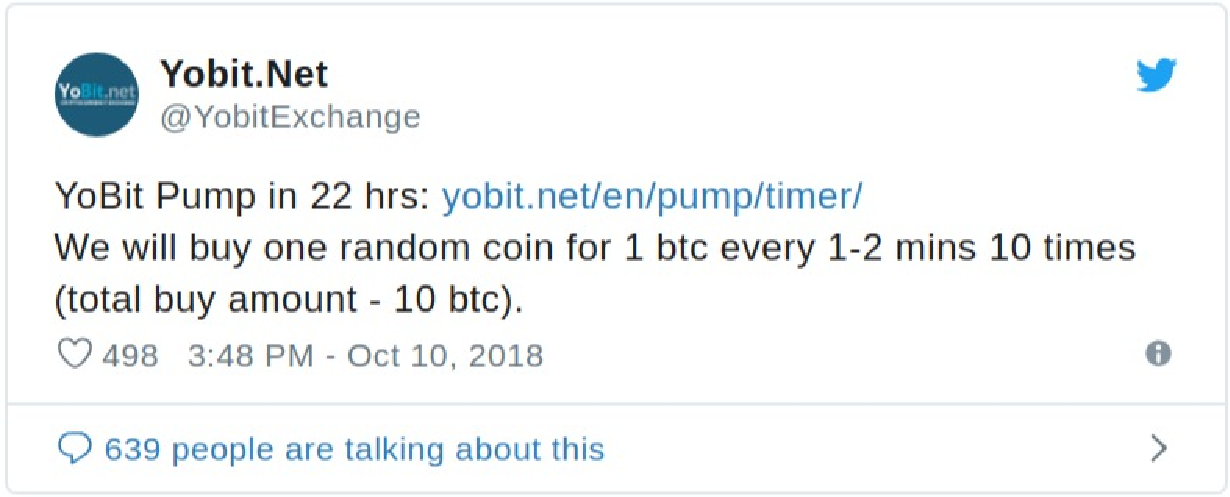
\includegraphics[width=\textwidth]{yobit.pdf}
    \caption{Yobit announcing a coin-pump through their official Twitter account}
    \label{fig:yobit}
\end{figure}

% Bittrex - banning pd

% kraken - low occurrences of pump and dump

% Binance - high volume, - lots of markets - appealing
